\documentclass{beamer}
\usepackage[utf8]{inputenc}
\usepackage{graphicx}
\usepackage{tabularx}
\usepackage[backend=biber, style=verbose]{biblatex}
\addbibresource{references.bib}


\title{Presentation of Potential of artificial intelligence in reducing energy and carbon emissions of commercial buildings at scale}
\author{Dwayne Mark Acosta (300665276) \\ Mohamed Amine Benaziza (300684553) \\ David Franz (300360491) \\ Ray Marange (300671115) \\ James Thompson (300680096)}
\date{\today}

\begin{document}

\frame{\titlepage}

\begin{frame}{Introduction}
\framesubtitle{Presented by: Ray Marange}

This summary reviews the paper by Chao Ding, Jing Ke, Mark Levine, and Nan Zhou titled \textit{Potential of Artificial Intelligence in Reducing Energy and Carbon Emissions of Commercial Buildings at Scale} \cite{dingPotentialArtificialIntelligence2024}.


\end{frame}

\begin{frame}{Introduction}
\framesubtitle{Presented by: Ray Marange}

\begin{itemize}
    \item Climate change is intensifying, and buildings are major contributors—accounting for 39\% of U.S. primary energy use.
    \item With urbanisation accelerating and building stock projected to double by 2060, improving building efficiency has become a critical global priority.
    \item While AI has transformed sectors like healthcare and finance, its application in building energy management remains limited.
    \item The paper outlines how AI can reduce costs, extend lifecycle benefits, and improve safety across the building lifecycle.
    \item This study focuses on medium-sized office buildings to examine AI’s capacity to reduce energy usage and carbon emissions.
    \item It presents a scalable framework with global applicability, making its insights relevant across diverse building contexts.
    \item Though centred on medium-sized offices, the findings are generalisable to commercial buildings of various sizes.
\end{itemize}

\end{frame}

\begin{frame}{Results part 1}
\framesubtitle{Presented by: Dwayne Mark Acosta}
\begin{itemize}
    \item According to the 2012 U.S. Energy Information Association (EIA), office buildings account for 20\% of commercial energy use.
    \item Median Energy Use Intensity (EUI) of typical office buildings: \textbf{167~kWh/m\textsuperscript{2}} (\textit{EUI\textsubscript{base}}).
    \item Verified low-energy office buildings (\textit{EUI\textsubscript{HEEB}}) achieve: \textbf{57~kWh/m\textsuperscript{2}}.
    \item This yields a Technical Energy Efficiency Saving (TEES) of: \textbf{110~kWh/m\textsuperscript{2}}.
    \item TEES is broken into four key optimization categories:
    \begin{enumerate}
        \item Equipment efficiency
        \item Occupancy influence
        \item Control and operation
        \item Design and construction
    \end{enumerate}
\end{itemize}
\end{frame}

\begin{frame}{Results Part 1}
\framesubtitle{Presented by: Dwayne Mark Acosta}

\begin{itemize}
    \item Medium office buildings make up \textbf{70\%} of total U.S. office energy consumption.
    \item The study used DOE's EnergyPlus tool, based on ASHRAE 90.1, to simulate annual energy use.
    \item Simulations covered four U.S. climate zones (1A, 3B, 4A, 5A) using representative cities.
    \item Natural gas was assumed for heating and hot water, electricity for all other loads.
    \item A total of \textbf{24 improvement cases} were modeled:
    \begin{itemize}
        \item 9 cases for equipment efficiency
        \item 9 cases for design and construction
        \item 6 cases for occupancy behavior and control
    \end{itemize}
\end{itemize}
\end{frame}

\begin{frame}{Results Part 1 – Equipment Efficiency}
    \framesubtitle{Presented by: Dwayne Mark Acosta}
    
    \scriptsize
    \begin{table}[h]
    \centering
    \caption{Equipment Efficiency Improvement Cases}
    \resizebox{\linewidth}{!}{
    \begin{tabularx}{\linewidth}{|c|X|X|}
    \hline
    \textbf{Case} & \textbf{Improvements} & \textbf{Adjustments} \\
    \hline
    E1 & HVAC – Cooling & +20\% \\
    E2 & HVAC – Heating & +12\% \\
    E3 & HVAC – Cases E1 and E2 & +20\%, +12\% \\
    E4 & Lighting – Power density (LPD) & -15\% \\
    E5 & Lighting – Power density (LPD) & -21\% \\
    E6 & Equipment – Power density (EPD) & -10\% \\
    E7 & Equipment – Power density (EPD) & -20\% \\
    E8 & Combined – Cases E1–E7 & \\
    E9 & Case E8 + Heat Pump for space heating & \\
    \hline
    \end{tabularx}
    }
    \end{table}
    \end{frame}

\begin{frame}{Results Part 2 – Design and Construction}
    \framesubtitle{Presented by: Dwayne Mark Acosta}
    
    \scriptsize
    \begin{table}[h]
    \centering
    \caption{Design and Construction Improvement Cases}
    \resizebox{\linewidth}{!}{
    \begin{tabularx}{\linewidth}{|c|X|X|}
    \hline
    \textbf{Case} & \textbf{Improvements} & \textbf{Adjustments} \\
    \hline
    D1 & Orientation & East (90° rotation) \\
    D2 & Orientation & South (180° rotation) \\
    D3 & Orientation & West (270° rotation) \\
    D4 & Envelope (walls, slabs, roofs, windows) & High insulation \\
    D5 & Envelope (walls, slabs, roofs, windows) & Increased infiltration (~60\%) \\
    D6 & Window-to-wall ratio (WWR) & Variation 1 \\
    D7 & Window-to-wall ratio (WWR) & Variation 2 \\
    D8 & Window-to-wall ratio (WWR) & Variation 3 \\
    D9 & Combined – Orientation, insulation, WWR & \\
    \hline
    \end{tabularx}
    }
    \end{table}
    \end{frame}

\begin{frame}{Results Part 3 – Occupant Behavior and Control}
    \framesubtitle{Presented by: Dwayne Mark Acosta}
    
    \scriptsize
    \begin{table}[h]
    \centering
    \caption{Occupant Behavior and Control Improvement Cases}
    \resizebox{\linewidth}{!}{
    \begin{tabularx}{\linewidth}{|c|X|X|}
    \hline
    \textbf{Case} & \textbf{Improvements} & \textbf{Adjustments} \\
    \hline
    B1 & Ventilation control & Open/close windows \\
    B2 & Lighting use & Switch on/off lights \\
    B3 & Electricity consumption & Turn off plug loads \\
    B4 & Lighting use & Dim lights \\
    B5 & HVAC & Turn on/off HVAC systems \\
    B6 & Thermostat & Adjust thermostat settings \\
    \hline
    \end{tabularx}
    }
    \vspace{0.5em}
    \textbf{Estimated Energy Savings:}
    \begin{itemize}
        \item Equipment: 11.5--17.3\%
        \item Design and Construction: 5.9--9.1\%
        \item Occupancy and Control: 15--20\%
    \end{itemize}
    \end{table}
    \end{frame}


\begin{frame}{Integrated Technical Energy-Saving Potential}
    \framesubtitle{Presented by: Dwayne Mark Acosta}
    
    \begin{figure}
        \centering
        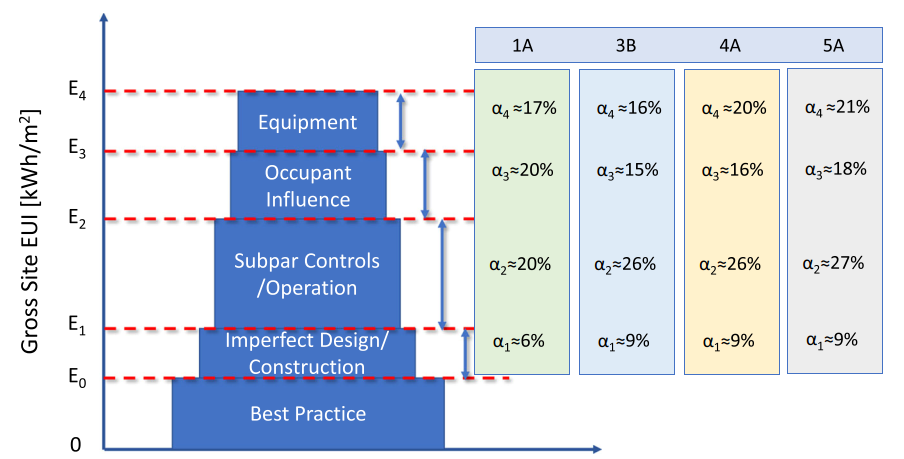
\includegraphics[width=0.95\textwidth]{figures/Integrated technical building energy-saving potential of a typical medium office building in the United States.png}
        \caption{Energy-saving potential by category across U.S. climate zones.}
        \label{fig:category-breakdown}
    \end{figure}
    \end{frame}
    

\begin{frame}{Results part 2}
\framesubtitle{Presented by: David Franz}


\end{frame}

\begin{frame}{Discussions}
\framesubtitle{Presented by: Mohamed Amine Benaziza}

Method \& scope
\begin{itemize}
    \item Mixed classic engineering with energy-simulation software (no single “magic” AI
tool).
    \item Tested on a medium-size office, but the same method works for hotels, malls, etc.
\end{itemize}
Why AI helps
\begin{itemize}
    \item Learns from building data to pick cheaper, better-fit efficiency fixes.
    \item Future add-ons (deep learning, reinforcement learning) promise even smarter control.
\end{itemize}

\end{frame}

\begin{frame}{Discussions}
\framesubtitle{Presented by: Mohamed Amine Benaziza}

Key numbers for U.S. medium offices
\begin{itemize}
    \item Four-part savings analysis (equipment, controls, occupants, design) shows
the theoretical max each climate zone can hit.
    \item AI alone vs. Business-as-usual 2050 $\to$ about 8 \% less energy \& CO$_2$.
    \item AI + existing efficiency policies $\to$ 19 \% extra cuts beyond policy alone.
    \item AI + strong policies + clean power (LEPG) $\to$ up to 40 \% less energy and 90 \% less CO$_2$ vs BAU.
\end{itemize}

\end{frame}

\begin{frame}{Discussions}
\framesubtitle{Presented by: Mohamed Amine Benaziza}

Limits \& take-aways
\begin{itemize}
    \item Results hinge on how fast costs fall and buildings adopt AI; other building types still need testing.
    \item Big idea: AI’s value is making proven high-efficiency designs affordable and widespread.
    \item Policy punchline: AI gets single-digit gains by itself; the huge drops only arrive when paired with clean-power policies and clear rules.
    \item Scaling to other sectors will need more research and skilled facility teams.
\end{itemize}

\end{frame}

\begin{frame}{Methods}
\framesubtitle{Presented by: James Thompson}

Two calculations used in this study. Lines up with 
\pause
\begin{itemize}[<+->]
    \item \textbf{Calculating potential savings}: simple model which is just summation of potential saving from each 4 categories
    \item \textbf{Calculating market share of low and no energy buildings}: more complicated and done by calculating the market share of each building type over time.
\end{itemize}
\end{frame}

\begin{frame}{Methods}
\framesubtitle{Presented by: James Thompson}

Calculation of the market share of different building types over time requires three things.
\begin{itemize}[<+->]
    \item The building type and its availability\\
    There is a limit on the Net Zero market share which is from 59\% - 79\%, depending on policy and AI use. Estimates are based off of other studies.
    \item The cost of the different building type\\
    High energy efficient buildings and Net Zero energy building cost more than standard buildings, around 10\%-20\% more. Calculated from construction data.
    \item The reduction in cost of the building over time.
    The cost premium of HEEB and NZEB building is assumed decreased over time, with decreases of 60\%-90\% depedning on scenarios. AI is just assumed to reduce cost premium by 10\%, the effects of policy and autonomous decreasing is unreferenced.
\end{itemize}
    
\end{frame}

\end{document}
